

\textbf{Fuktionsweise} Mit einem Laser wird der Schnee sowohl durchleuchtet für die Refraktion als auch angeleuchtet für die Reflexion. Flüssiges Wasser bildet aufgrund seiner Oberflächenspannung konkave Linsen auf den Prismen der Eiskristalle. Die Grösse und damit die Brennweite ändern sich je nach dem, wie viel Volumen Wasser auf den Eiskristallen ist. Die Effekte der Linsen sollten in der Refraktion sichtbar werden.

In der Reflexion ändert sich mit änderndem LWC auch die Oberfläche, an der das Licht gespiegelt wird. Der TRL für Refraktion und Reflexion ist bei 2.


\textbf{Beispiele in anderen Sektoren}
RRefraktion wird in der Kristallografie angewendet. Die Reflexion wird bei einem Auflichtmikroskop fast immer angewendet wird. Die Reflexion von Wasser an einer Glasscheibe wird genutzt, um bei Autos Niederschlag auf der Windschutzscheibe zu messen. In den drei Fällen ist das TRL 9.

\textbf{Literatur zu Reflexion}
Die Publikation \cite{} hat den LWC mit der Reflexion von IR-EM Wellen bestimmt.

\textbf{Benutzte Mittel für den Versuchsaufbau}
Als Laserquelle wurde ein grüner Bosch Quingo Kreuzlaser genutzt. Um sowohl die Reflexion als auch die Refraktion gleichzeitig zu sehen, wurde die Schneeprobe auf einen Mikroskopier-Objektträger platziert. Die Ergebnisse des Lasers wurden jeweils auf weissem Druckpapier dargestellt. Die Refraktion wird auf dem Papier an der Unterseite der Holzplatte dargestellt. Mit dem Fairphone 3 wurde eine Videoaufnahme gemacht, wie sich die Ergebnisse des Lasers verändern. Mit einem Kosmetikspiegel wurde sowohl die Reflexion unten als auch die Refraktion oben gleichzeitig in einem Bild dargestellt. Um alle Teile in festen Relationen zu halten, wurde Stativmaterial genutzt.



In Bild \ref{fig:LaserAufbau} ist die Anordnung der Verschieden Teile auf den Stativmaterial zu sehen.


\begin{figure}
    \centering
    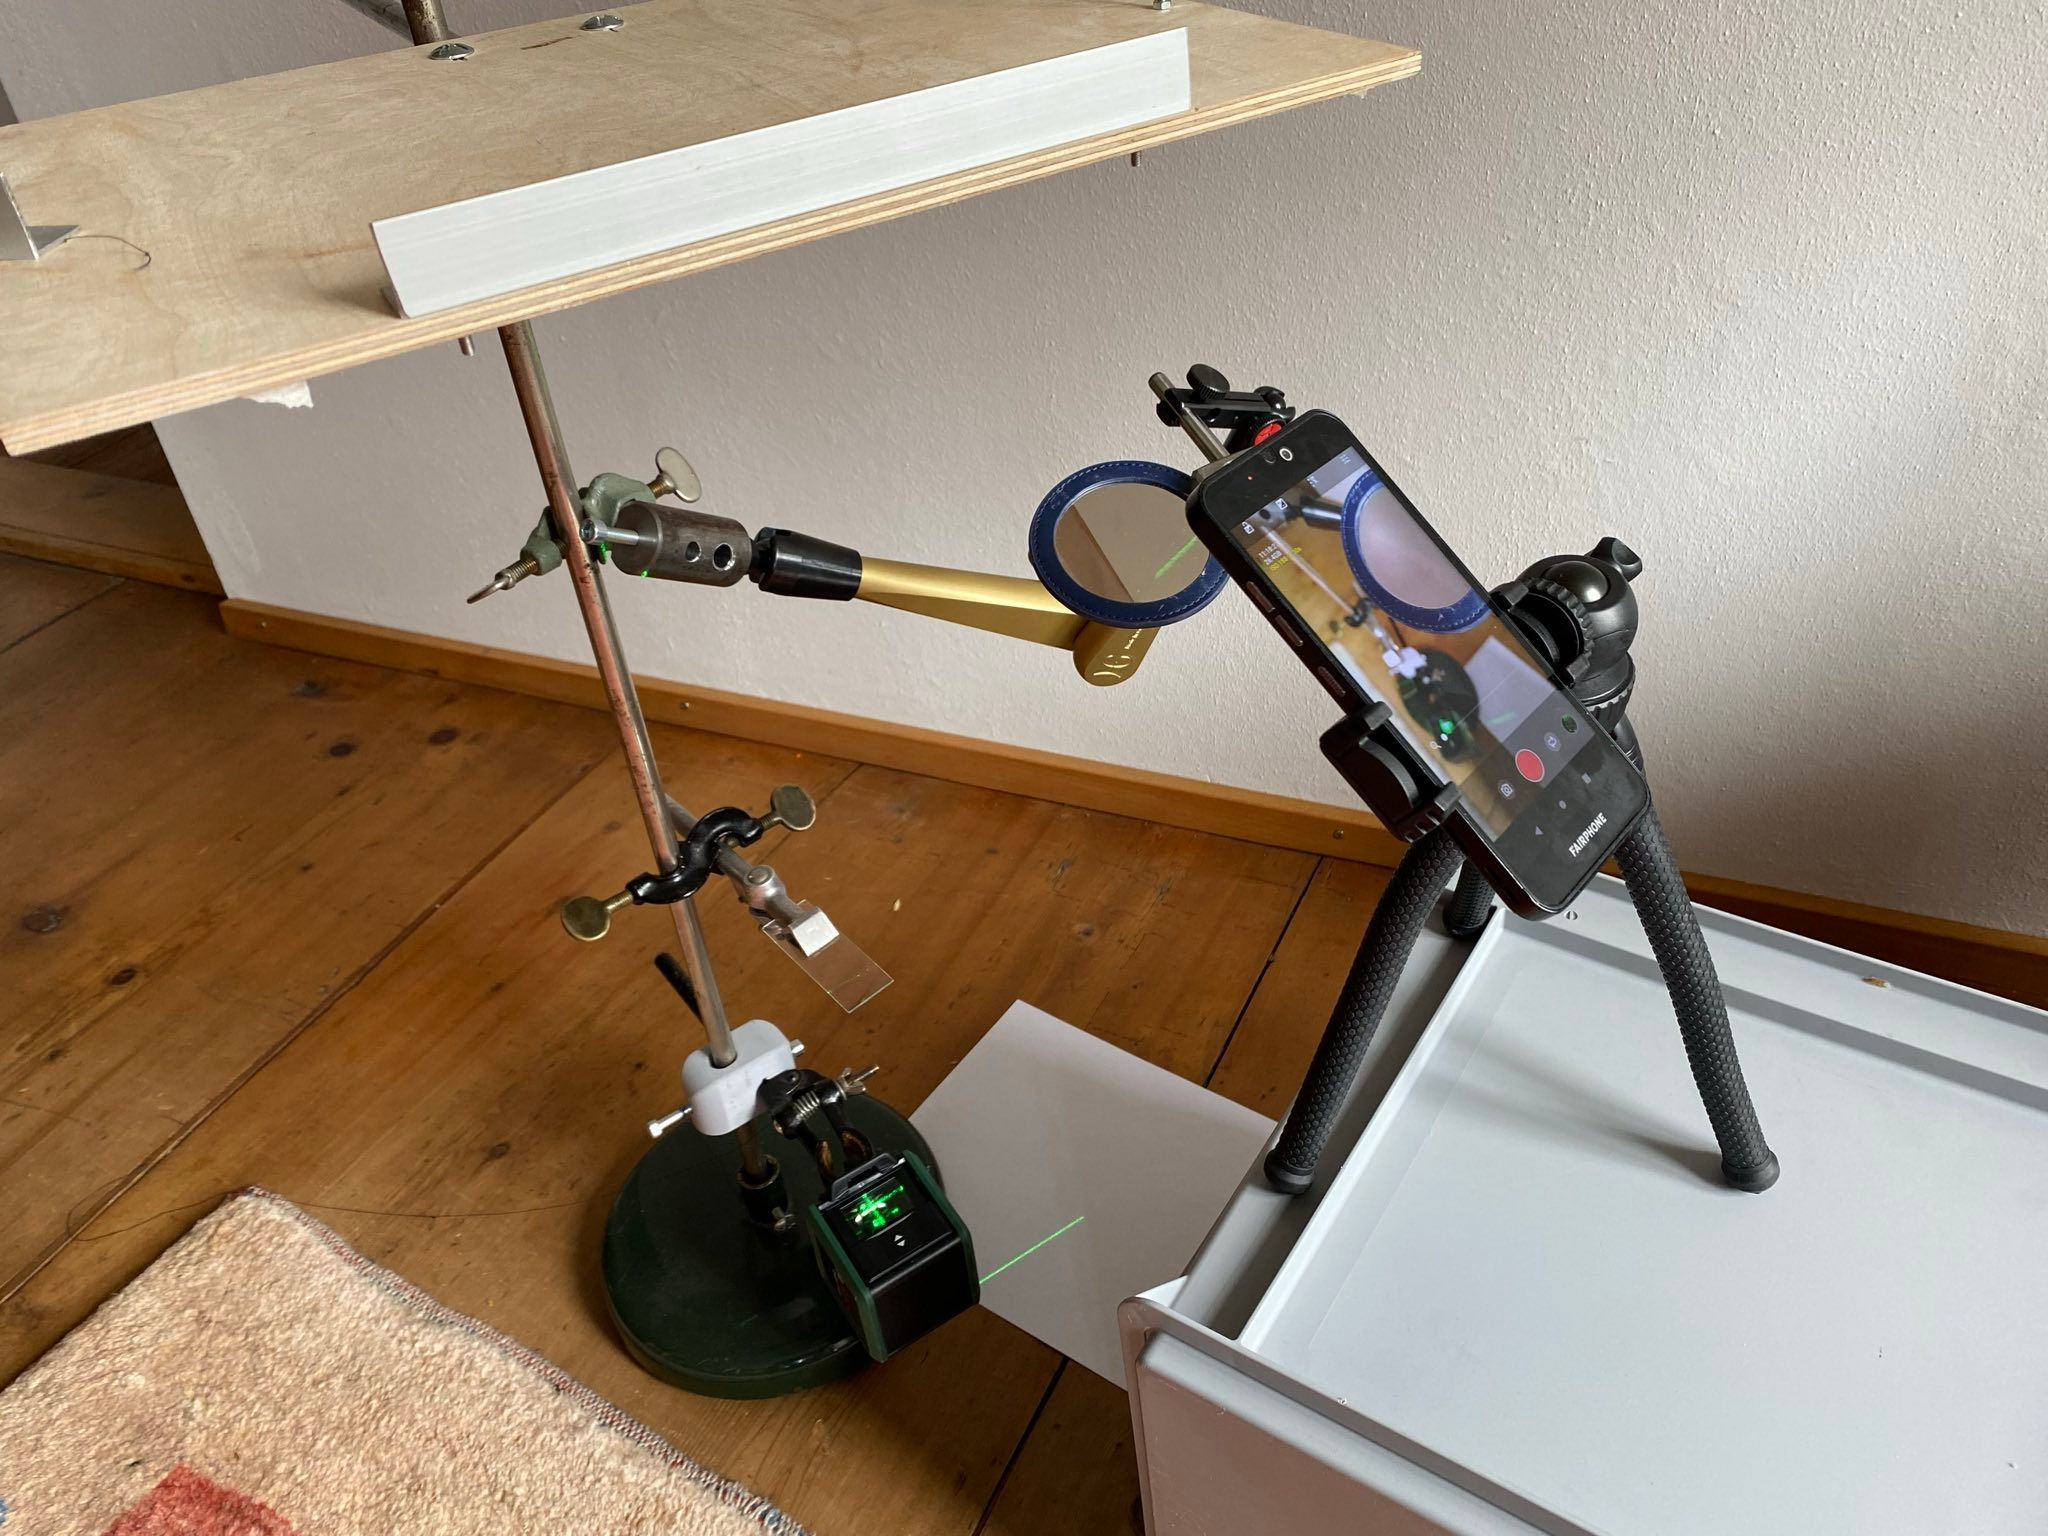
\includegraphics[width=0.8\textwidth]{Bilder/signal-2024-03-10-112013_006.jpeg}
    \caption{Versuchsaufbau der Laser Reflexion und Refraktion}
    \label{fig:LaserAufbau}
\end{figure}


\textbf{Funktionsweise des Versuchsaufbaus}
Der Schnee wird im trockenen Zustand bei -10 Grad Celsius aus dem Gefrierschrank auf den gekühlten Objektträger gelegt. Dann wird beobachtet, wie sich die Ergebnisse ändern, wenn der Schnee an der Raumtemperatur schmilzt. Dieser Schmelzvorgang dauerte rund 3 Minuten. Der Laser scheint durch den Objektträger und den Schnee hindurch, dann wird das Licht auf das Papier erneut in die Kamera reflektiert. Die Reflexion geschieht zum einen direkt am Objektträger, als auch danach im Schnee. Dieser Aufbau ist suboptimal, denn die konstante Reflexion des Objektträgers muss aus dem Laserergebnis herausgerechnet werden. Um Störlicht zu minimieren, wurde zuerst eine Einhausung geplant. Der durchgeführte Versuch hat dann aber einfach in einem abgedunkelten Raum stattgefunden.


\begin{figure}[h]
    \centering
    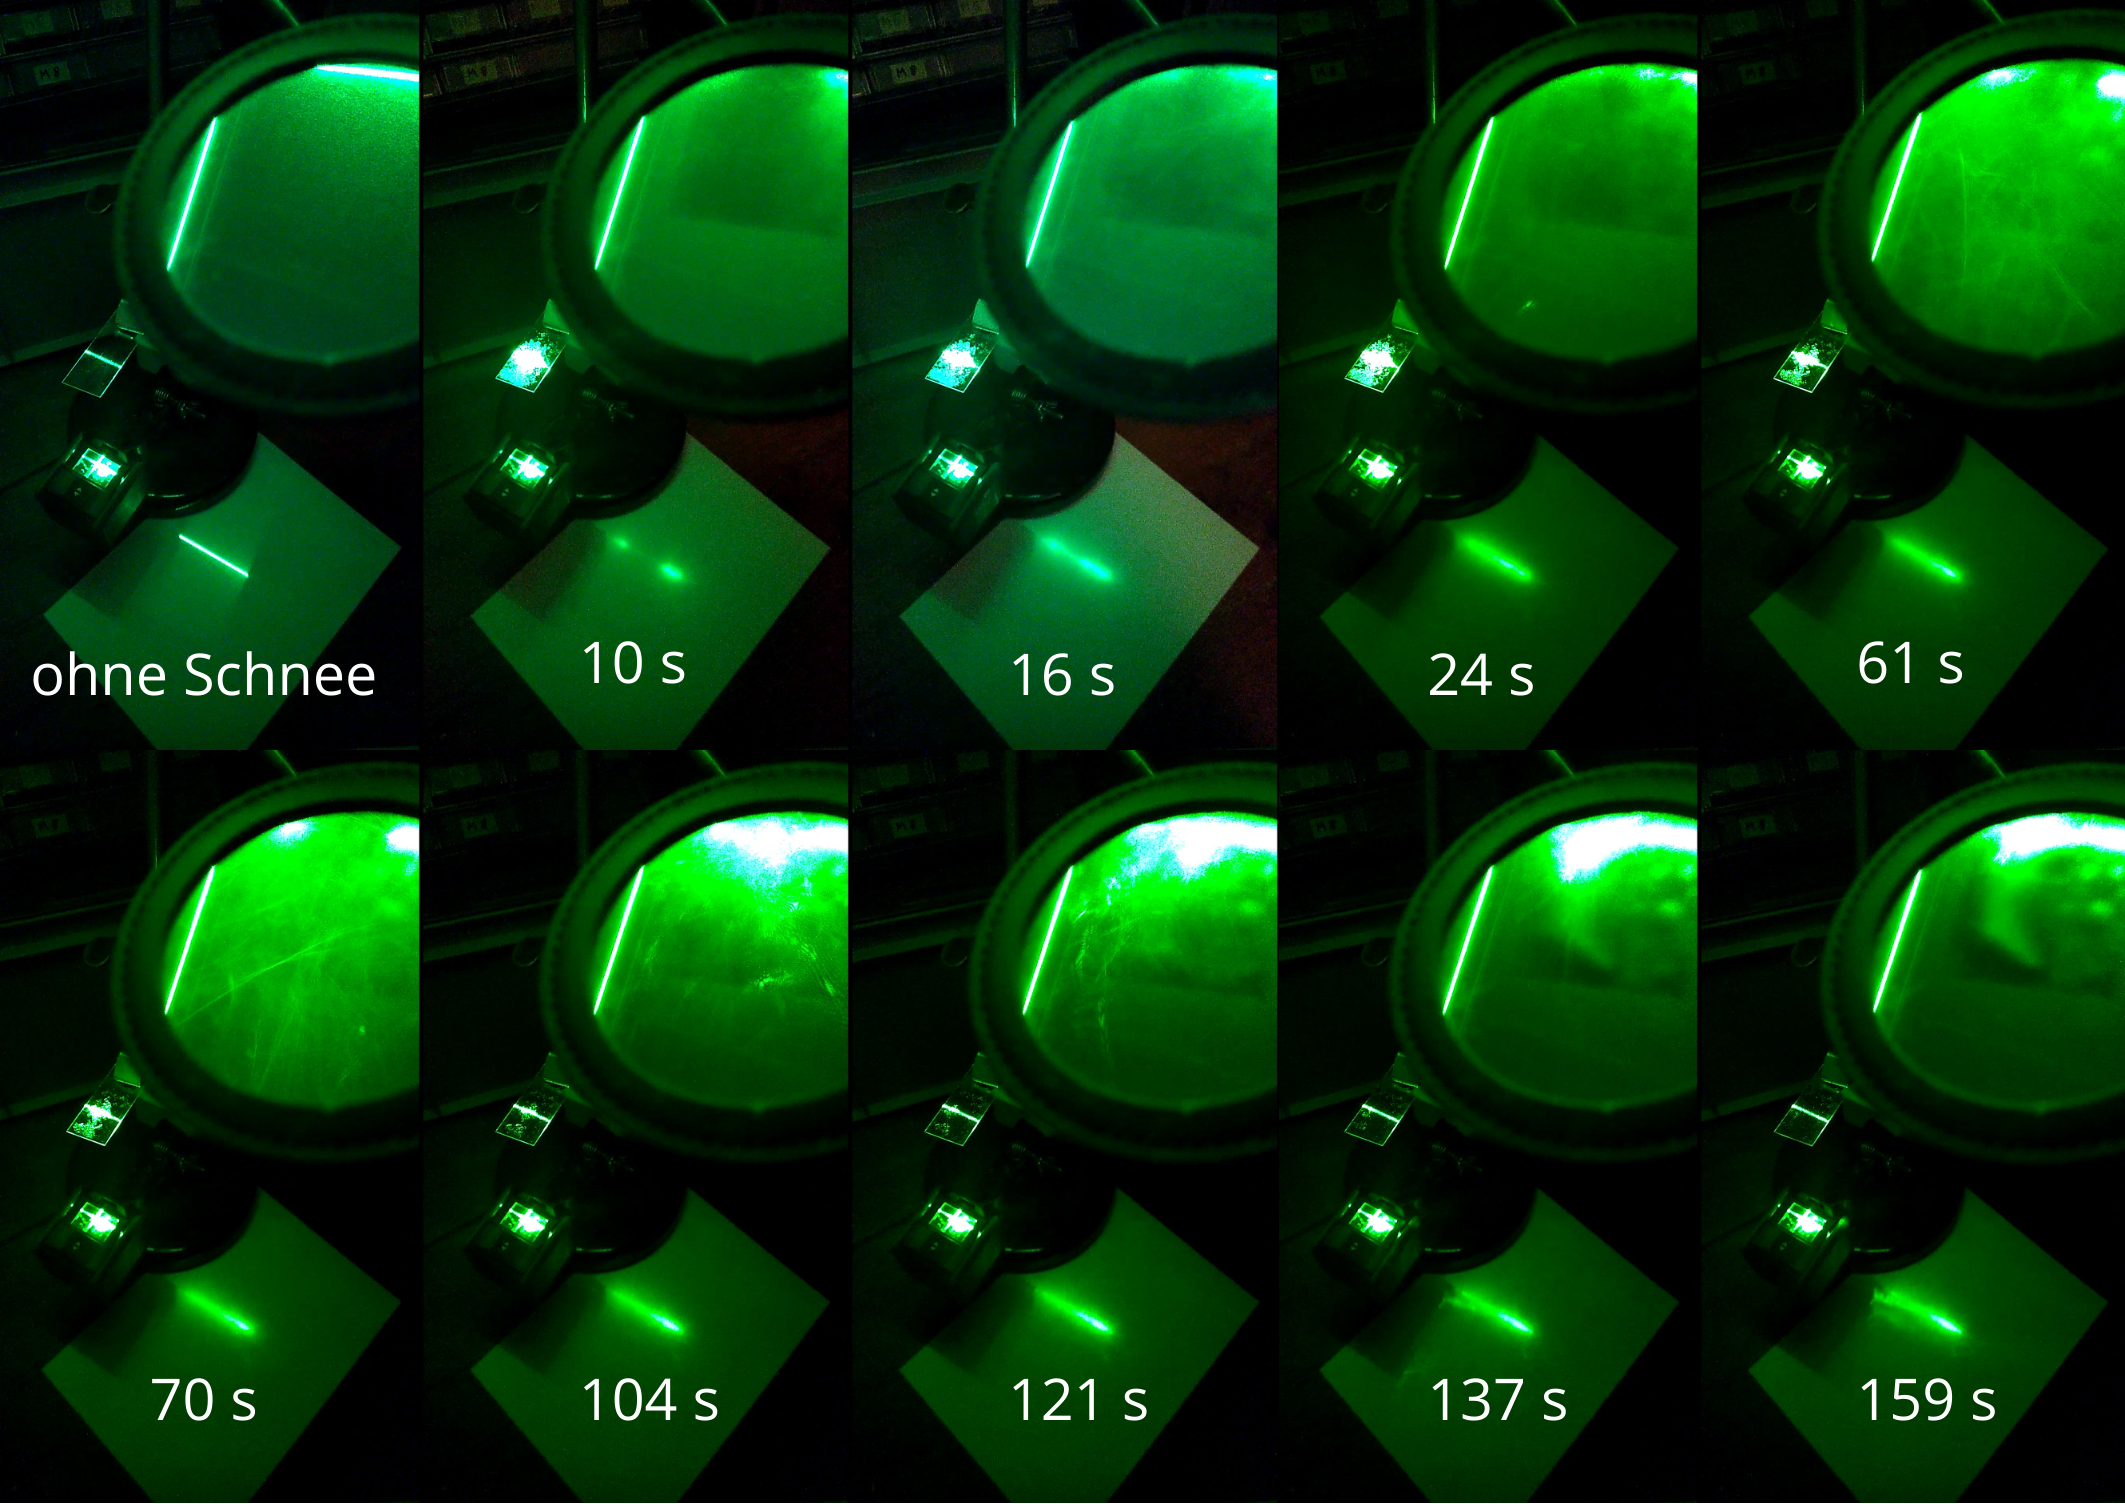
\includegraphics[width=0.8\textwidth]{Bilder/Screenshotfrom2024-04-0413-27-28.png}
    \caption{Messgrössen für die Reflexion und Refraktion, Veränderung über Zeit}
    \label{fig:LaserRef}
\end{figure}



\textbf{Messgrössen}
Die Anhäufungen von Licht und die Intensität können begutachtet werden.

\textbf{Versuchsergebnisse}
Im Bild \ref{fig:LaserRef} ist die Reflexion und Refraktion des Objektträgers sichtbar. Diese konstanten Werte müssen von allen Ergebnissen subtrahiert werden.








\textbf{Aussagekraft der Ergebnisse über den LWC}
Die Ergebnisse werden direkt von Wasser beeinflusst. Um den Gewichts-LWC zu erhalten, ist aber die Geometrie der Eiskristalle von extremer Bedeutung. Daher ist das Ergebnis nicht direkt mit den LWC überführbar. Mit der 3D-Geometrie der Kristalle wäre die Aussagekraft besser.

\textbf{Reflexion zum Versuchsaufbau}
Da zwei Techniken gleichzeitig gemessen wurden, war der Versuchsaufbau nicht optimal für beide Messgrößen. Mit den Ergebnissen der Refraktion bin ich sehr zufrieden. Es ist eine klare Veränderung sichtbar.

\textbf{Verbesserungen des Versuchsaufbaus}
Um bessere Reflexionsergebnisse zu bekommen, keinen Objektträger nutzen, sondern direkt auf Schnee leuchten. Für eine statische Messung einer Schneeprobe muss die Luft um den Schnee herum gekühlt sein. Ein Ansatz dafür wird im Vorversuch \ref{sec:TinteVersuchsaufbau} umgesetzt. Mit dem Laser wird Energie in den Schnee eingebracht. Um das Schmelzen und damit Verfälschen des LWC zu minimieren, sollte ein möglichst schwacher Laser eingesetzt werden.

\textbf{Weiterverfolgung der physikalischen Methoden}
Das Ergebnis der Refraktion zeigt, dass diese Methode umgesetzt werden könnte. Um vergleichbare Werte zu bekommen, ist die Kristallgeometrie aber von Bedeutung. Die Messung der Geometrie übersteigt das Ausmaß der BA. Um eine Messung durchzuführen, muss eine Schneeprobe durchleuchtet werden. Um das zu erreichen, muss der Schnee physikalisch aus der Schneedecke extrahiert werden. Das ist aufwendig. Daher wird die Refraktion nicht weiterverfolgt. Das Ergebnis der Reflexion ist schwer zu beurteilen. In \ref{sec:PubMeth} ist die Reflexion von EM-Wellen bereits untersucht worden. Daher wird die Reflexion nicht weiter untersucht.
